\documentclass[12pt, polish, aspectratio = 169]{beamer}
\usepackage{beamer}

\date{Wersja \gitVer{} z \today{}}
\title{Rozprawa Doktorska}
\author{mgr inż. Łukasz Dróżdż}
\subject{Analiza metrologiczna algorytmów dyskretnej transformacji falkowej}
\subtitle{Analiza metrologiczna algorytmów dyskretnej transformacji falkowej}
\institute{Politechnika Śląska, Wydział Elektryczny \\ Katedra Metrologii, Elektroniki i Automatyki}
\keywords{dyskretna transformacja falkowa, cyfrowe przetwarzanie sygnałów, szacowanie niepewności wyniku pomiaru, analiza właściwości metrologicznych toru pomiarowego}

\begin{document}

\section*{Wstęp}

\begin{frame}
\titlepage
\end{frame}

\begin{frame}{Plan prezentacji}
\tableofcontents
\end{frame}

\section{Przedstawienie tezy pracy oraz jej najważniejszych założeń}

\begin{frame}{Teza pracy}
\justifying
Stosując przedstawiony w pracy model błędów oraz zaproponowaną metodę szacowania wypadkowej wartości niepewności rozszerzonej istnieje możliwość oszacowania wartości niepewności rozszerzonych dla wielkości wyjściowych toru pomiarowego wykorzystującego algorytm dyskretnej transformacji falkowej.

Oszacowanie wartości niepewności rozszerzonych dla omawianych wielkości jest możliwe w trakcie działania systemu pomiarowego, również w przypadku zmiany parametrów pracy tego systemu i wynikającej z tego tytułu zmiany parametrów modelu błędów.

Skuteczność zaproponowanej metody szacowania wypadkowej wartości niepewności rozszerzonej wynika z dokładności określenia parametrów modelu błędów, a uzyskiwane wyniki są zbieżne z uzyskiwanymi metodą Monte-Carlo.
\end{frame}

\begin{frame}{Podsumowanie tezy}
\begin{itemize}
\item Propozycja modelu błędów umożliwiającego opis właściwości metrologicznych torów pomiarowych wykorzystujących algorytmy transformacji falkowej
\item Propozycja metody szacowania wartości wypadkowej niepewności rozszerzonej, która:
	\begin{itemize}
	\item cechuje się niską złożonością obliczeniową i jest możliwa do stosowania w czasie pracy systemu pomiarowego
	\item daje możliwość zmiany parametrów modelu błędów podczas pracy systemu pomiarowego, zachowując niską złożoność obliczeniową
	\end{itemize}
\item Wyniki uzyskiwane przy użyciu zaproponowanej metody powinny być zbieżne z wynikami uzyskiwanymi metodą Monte-Carlo
\item Dokładność uzyskiwanych wyników może zależeć od dokładności wyznaczenia parametrów modelu błędu
\end{itemize}
\end{frame}

\section{Przedstawienie najważniejszych właściwości metrologicznych algorytmów transformacji falkowej}

\begin{frame}{Algorytm transformacji falkowej}
\begin{equation}
w_{a,b} = \frac{1}{\sqrt{a}} \int _{-\infty} ^{\infty} x \emb{t} \psi \emb{\frac{t-b}{a}} dt \label{eq:cwt}
\end{equation}
\begin{itemize}
\item Wykorzystuje funkcję \enquote{falki-matki}, oznaczoną jako $\psi(t)$
\item Umożliwia analizę sygnału $x(t)$ w dziedzinie skala-czas
\item Dla wybranej skali $a$ współczynniki transformacji $w_{a,b}$ wyznaczane są dla kolejnych okien pomiarowych, przesuniętych o czas $b$
\item Parametr skali $a$ określa zakres częstotliwości harmonicznych sygnału $x(t)$
\item Występuje w kilku głównych odmianach:
	\begin{itemize}
	\item[CWT] ciągła transformacja falkowa
	\item[DWT] dyskretna transformacja falkowa
	\item[UFWT] dyskretna transformacja falkowa bez decymacji
	\end{itemize}
\end{itemize}
\end{frame}

\begin{frame}{Obszary zastosowań algorytmu}
\begin{itemize}
\item Umożliwiają detekcję, czy zjawisko o określonym widmie częstotliwościowym miało miejsce w danym czasie
\end{itemize}
\begin{itemize}
\item Przetwarzanie, kompresja oraz analiza obrazów i dźwięków
\item Redukcja szumu w sygnale pomiarowym
\item Analiza sygnałów EKG oraz EEG
\item Analiza przebiegu drgań sejsmicznych
\item Bezinwazyjna analiza stanu elementów mechanicznych
\item Algorytmy stratnej kompresji danych
\item Analiza zwarć wysoko prądowych
\item Analiza procesów hydrologicznych
\end{itemize}
\end{frame}

\begin{frame}{Algorytm dyskretnej transformacji falkowej}
\begin{equation}
w_{m,n} = \frac{1}{\sqrt{2^{m}}} \int _{-\infty} ^{\infty} x \emb{t} \psi \emb{\frac{t - n 2^{m}}{2^{m}}} dt \label{eq:dwt}
\end{equation}
\begin{itemize}
\item Wyznaczenie nieskończonej liczby współczynników transformacji jest niemożliwe, a wyznaczanie nadmiarowej liczby współczynników transformacji nie jest konieczne w celu analizy i rekonstrukcji sygnału
\item Wprowadzenie ograniczenia dostępnych wartości dla parametrów skali $a$ oraz przesunięcia w czasie $b$, gdzie $a = 2^m$, $b = n2^m$ dla $m, n \in \mathbb{N}$ zapewnia:
	\begin{itemize}
	\item eliminację nadmiarowych współczynników transformacji $w_{m,n}$
	\item możliwość rekonstrukcji oryginalnego sygnału $x(t)$
	\item dynamiczną rozdzielczość podstawy czasu dla kolejnych skal
	\end{itemize}
\item Symbol $m$ oznacza numer skali (zakres częstotliwości)
\item Symbol $n$ oznacza numer okna pomiarowego
\end{itemize}
\end{frame}

\begin{frame}{Algorytm dyskretnej transformacji falkowej}
\begin{itemize}
\item Dla kolejnych numerów skali algorytm stanowi filtr pasmowo-przepustowy, którego częstotliwość charakterystyczna zmniejsza się w stosunku do poprzedniego numeru skali o połowę
\item W celu wyodrębnienia z sygnału wszystkich zakresów częstotliwości należy wyznaczyć współczynniki transformacji dla nieskończonej liczby skal
\item Jako, że to niemożliwe, stosuje się funkcję skalującą, która tworzy filtr dolno-przepustowy, przenoszący pozostałą cześć widma sygnału
\item Funkcja skalująca, zwana również \enquote{falką-ojcem}, musi być zdefiniowana dla stosowanej funkcji \enquote{falki-matki} i jest oznaczana symbolem $\phi(t)$
\end{itemize}
\end{frame}

\begin{frame}{Algorytm dyskretnej transformacji falkowej}
\begin{itemize}
\item Proces dekompozycji sygnału przeprowadzany jest rekurencyjnie w celu wyznaczenia wartości współczynników transformacji dla kolejnych wartości parametru skali (rys.~\ref{fig:fwt_decomp})
\item Zwykle nie jest znana bezpośrednia postać funkcji falki-matki $\psi(t)$ oraz funkcji skalującej $\phi(t)$ w dziedzinie czasu -- zdefiniowane są \enquote{współczynniki skalujące} $c_{k}$ umożliwiające opis funkcji $\psi_{m,n}(t)$ oraz $\phi_{m,n}(t)$
\item Dla wybranej rodziny falek istnieje możliwość stworzenia falki o zadanym rzędzie oraz wykonanie dowolnej* liczby iteracji procesu dekompozycji
\item Podczas projektowania toru pomiarowego często zachodzi potrzeba zmiany parametrów algorytmu, w tym zmiany falki-matki, jej rzędu, liczby iteracji procesu dekompozycji sygnału, czy liczby próbek wielkości wejściowej
\end{itemize}
\end{frame}

\begin{frame}{Proces dekompozycji sygnału}
\begin{figure}
\includegraphics[scale = 0.75]{obrazki/dwt_dekompozycja}
\caption{Przykład trzech iteracji procesu dekompozycji sygnału}
\label{fig:fwt_decomp}
\end{figure}
\begin{itemize}
\item $S_{0}$ to kolejne próbki przetwarzanego sygnału $x(i)$
\item $S_{m}$ to kolejne próbki aproksymacji sygnału dla skali $m$
\item $T_{m}$ to kolejne próbki detali sygnału dla skali $m$
\end{itemize}
\end{frame}

\begin{frame}{Bank filtrów algorytmu}
\begin{figure}
\includegraphics[scale = 0.75]{obrazki/bank_db_short}
\caption{Przykładowe banki filtrów dla rodziny \enquote{Daubechies}, częstotliwość znormalizowano do połowy częstotliwości próbkowania, wartość wzmocnienia znormalizowano do maksymalnej wartości wzmocnienia dla każdego filtru z osobna}
\end{figure}
\end{frame}

\begin{frame}{Właściwości metrologiczne algorytmu}
\begin{itemize}
\item Algorytm przetwarza sygnały błędów obecne w sygnale wejściowym zgodnie z charakterystyką banku filtrów
\item Rzeczywista implementacja algorytmu wprowadza błędy własne, związane z operacjami arytmetycznymi
\item Proponowane w literaturze metody analizy są skomplikowane, a dodatkowo ich aplikacja w przypadku zmiany parametrów algorytmu wiąże się z powtórnym procesem analizy, co jest czasochłonne
\item Nie zawsze znane są jawne postaci funkcji falki-matki $\psi(t)$ oraz funkcji skalującej $\phi(t)$ dla wybranej rodziny, co utrudnia analizę
\item Projektant toru pomiarowego nie jest zwykle ekspertem z dziedziny falek, a jedynie użytkownikiem stosującym gotową implementację algorytmu
\end{itemize}
\end{frame}

\begin{frame}{Błędy własne algorytmu}
\begin{equation}
e_{X,z} \emb{j} = \tilde{X} \emb{j} - \dot{X} \emb{j} \label{eq:fwt_outerr_self}
\end{equation}
\begin{itemize}
\item Sygnał błędu własnego $e_{X,z}(j)$ związany z $j$-tą wielkością wyjściową wynika z zaokrągleń wykonywanych podczas operacji arytmetycznych
\item Parametry sygnału błędu własnego zaokrągleń powinny być wyznaczane dla rzeczywistej implementacji algorytmu o wybranych parametrach
\item Eksperyment należy przeprowadzić zakładając, że wielkości wejściowe $x(i)$ algorytmu nie są obarczone żadnymi błędami, zatem $\tilde{x}(t) = \dot{x}(t)$
\item Dla algorytmu idealnego sygnał ten nie występuje, wtedy $e_{X,z}(j) = 0$
\end{itemize}
\end{frame}

\begin{frame}{Błędy własne algorytmu}
\begin{figure}
\includegraphics[scale = 0.75]{obrazki/schemat_dwt_ew}
\caption{Schemat blokowy procedury wyznaczania pojedynczej realizacji sygnału błędu własnego $e_{X,z}(j)$ algorytmu transformacji falkowej}
\end{figure}
\end{frame}

\begin{frame}{Wariancja sygnału błędu własnego zaokrągleń}
\begin{figure}
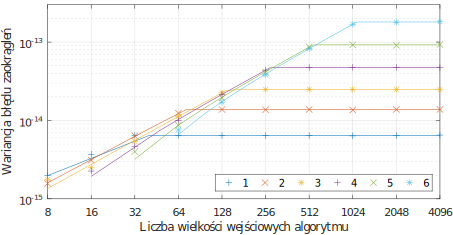
\includegraphics[scale = 0.75]{obrazki/dwt_rerror_coif5}
\caption{Wartość wariancji sygnału błędu $e_{X,z}(j)$ w funkcji wybranych parametrów algorytmu DWT, falka \enquote{coif5}, liczby o długości~\qty{32}{\bitOw}, ostatni etap dekompozycji}
\end{figure}
\end{frame}

\begin{frame}{Wariancja sygnału błędu własnego zaokrągleń}
\begin{itemize}
\item Zależy od liczby przeprowadzanych operacji arytmetycznych, a zatem:
	\begin{itemize}
	\item wzrasta wraz ze wzrostem liczby iteracji procesu dekompozycji sygnału
	\item wzrasta wraz ze wzrostem rzędu falki
	\item wzrasta wraz ze wzrostem liczby wielkości wejściowych
	\end{itemize}
\item Zależy od długości słowa liczb zmiennoprzecinkowych
\item Zależy od zakresu wartości wielkości wejściowych
\item Powinna być wyznaczana w warunkach zbliżonych do warunków pracy rzeczywistego algorytmu
\item Długość słowa należy dobrać tak, aby wariancja sygnału błędu własnego była niewielka w stosunku do wariancji wypadkowego sygnału błędu przetwarzanych wielkości
\end{itemize}
\end{frame}

\section{Omówienie najważniejszych założeń odnośnie zaproponowanego w pracy modelu błędów}

\begin{frame}{Podstawowe założenia modelu błędów}
\begin{itemize}
\item Możliwość analizy sygnałów błędów opisanych deterministycznie i niedeterministycznie
\item Uwzględnienie wpływu widma przetwarzanego sygnału na właściwości metrologiczne toru pomiarowego
\item Sygnał błędu opisany jako różnica pomiędzy idealnym i rzeczywistym przebiegiem analizowanej wielkości
\item Idealny przebieg analizowanej wielkości wynika z założeń odnośnie realizowanego przez tor pomiarowy zadania
\item Każdy fragment toru pomiarowego przetwarza sygnały błędów obecne w sygnale wejściowym oraz wprowadza sygnały błędów własnych
\item Tor pomiarowy może składać się z wielu obiektów przetwarzających ciągły w czasie sygnał lub kolejne próbki sygnału
\end{itemize}
\end{frame}

\begin{frame}{Podział sygnałów błędów}
\begin{itemize}
\item Podział sygnałów błędów ze względu na charakter realizacji:
	\begin{itemize}
	\item \strong{sygnały błędów statycznych}, których wartości realizacji nie zmieniają się dla analizowanej serii pomiarowej
	\item \strong{sygnały błędów dynamicznych}, których wartości realizacji zmieniają się dla analizowanej serii pomiarowej i są opisane deterministycznie
	\item \strong{sygnały błędów statycznych}, których wartości realizacji zmieniają się dla analizowanej serii pomiarowej zgodnie z regułami probabilistycznymi
	\end{itemize}
\item Podział sygnałów błędów ze względu na genezę:
	\begin{itemize}
	\item \strong{sygnały błędów własnych}, wprowadzanie przez analizowany obiekt
	\item \strong{sygnały błędów propagowanych}, przenoszone z wejścia na wyjście obiektu
	\end{itemize}
\item Termin \enquote{seria pomiarowa} odnosi się zwykle do pojedynczego okna pomiarowego lub zbioru próbek, stanowiących wejście dla pojedynczej realizacji algorytmu przetwarzania danych
\end{itemize}
\end{frame}

\begin{frame}{Model błędu toru pomiarowego}
\begin{figure}
\includegraphics[scale = 0.75]{obrazki/schemat_trans}
\caption{Schemat blokowy toru pomiarowego, na który przedstawiono proces wyznaczania wartości realizacji pojedynczej wielkości wyjściowej}
\end{figure}
\begin{itemize}
\item Wielkość fizyczna $s(t)$ jest przetwarzana na wielkość $y(t)$
\item Kolejne próbki wielkości $y(t)$ reprezentowane są przez wielkość $x(i)$
\item Na podstawie wielkości $x(i)$ wyznaczane są wartości wielkości $X(i)$
\end{itemize}
\end{frame}

\begin{frame}{Analizowane fragmenty toru pomiarowego}
\begin{itemize}
\item \strong{Część analogowa}, która przetwarza ciągły w czasie sygnał $s(t)$
\item \strong{Część cyfrowa}, która przetwarza próbki sygnału $y(t_{i})$
\item \strong{Przetwornik analogowo-cyfrowy}:
	\begin{itemize}
	\item zamienia ciągły w czasie sygnał $y(t)$ na jego dyskretną reprezentację $x(i)$
	\item opisywany jako kaskadowe połączenie modelu części analogowej, idealnego kwantyzatora oraz części cyfrowej
	\end{itemize}
\item Każdy fragment toru pomiarowego posiada właściwości:
	\begin{itemize}
	\item \strong{statyczne}, niezależne od widma przetwarzanego sygnału
	\item \strong{dynamiczne}, zależne od widma przetwarzanego sygnału
	\end{itemize}
\item Tor pomiarowy może składać się z wielu obiektów połączonych kaskadowo
\item Tor pomiarowy może dostarczać na wyjściu wiele wielkości wyjściowych
\end{itemize}
\end{frame}

\begin{frame}{Część analogowa toru pomiarowego}
\begin{figure}
\includegraphics[scale = 0.75]{obrazki/schemat_ciagly}
\caption{Model fragmentu części analogowej toru pomiarowego}
\end{figure}
\begin{itemize}
\item Obiekt przetwarza ciągłą w czasie wielkość $s(t)$ na wielkość $y(t)$
\item Właściwości dynamiczne opisuje transmitancja $G_{y}(j\omega)$
\item Właściwości statyczne opisuje funkcja przetwarzania $f_{y}(x)$
\item Przykładem obiektu może być filtr analogowy, przetwornik pomiarowy, wzmacniacz pomiarowy lub układ próbkująco-pamiętający
\end{itemize}
\end{frame}

\begin{frame}{Część analogowa toru pomiarowego}
\begin{itemize}
\item Parametry $G_{y}(j\omega)$ oraz $f_{y}(x)$ mogą być opisane:
	\begin{itemize}
	\item dla warunków idealnych, jako $\dot{G}_{y}(j\omega)$ oraz $\dot{f}_{y}(x)$
	\item dla warunków rzeczywistych, jako $\tilde{G}_{y}(j\omega)$ oraz $\tilde{f}_{y}(x)$
	\end{itemize}
\item Z uwagi na fakt, że rzeczywiste właściwości obiektu odbiegają od idealnych, obiekt wprowadza błędy własne
\item Obiekt przetwarza sygnały błędów zawarte w wielkości wejściowej zgodnie z jego rzeczywistymi właściwościami
\item Dla właściwości dynamicznych opisać można wzmocnienie $K_{y}(\omega)$ oraz przesunięcie fazowe $\varphi_{y}(\omega)$ w funkcji pulsacji $\omega$ jako:
\begin{gather}
K_{y} \emb{\omega} = \left| G_{y} \emb{j\omega} \right| =
	\sqrt{\left( \Re \left( G_{y} \emb{j\omega} \right) \right)^{2} +
	\left( \Im \left( G_{y} \emb{j\omega} \right) \right)^{2}}
\label{eq:mid_cont_amp}, \\
\varphi_{y} \emb{\omega} = \arctan \left( \frac{\Im \left( G_{y} \emb{j\omega} \right)}{\Re \left( G_{y} \emb{j\omega} \right)} \right) \label{eq:mid_cont_phi}.
\end{gather}
\end{itemize}
\end{frame}

\begin{frame}{Część analogowa toru pomiarowego}
\begin{itemize}
\item Wielkość wejściowa $s(t)$ w przypadku idealnym opisana równaniem:
\begin{equation}
\dot{s} \emb{t} = \sum _{i = 0} ^{\infty} E_{s,o} \emb{\omega_{i}} \sin \left( \omega_{i} t + \varphi_{s,o} \emb{\omega_{i}} \right) \label{eq:in_cont_omega_ideal}
\end{equation}
\item Wielkość wyjściowa $y(t)$ w przypadku idealnym opisana jako:
\begin{equation}
\dot{y} \emb{t} = \dot{f}_{y} \emb{ \sum _{i = 0} ^{\infty} \dot{K}_{y} \emb{\omega_{i}} E_{s,o} \emb{\omega_{i}} \sin \left( \omega_{i} t + \varphi_{s,o} \emb{\omega_{i}} + \dot{\varphi}_{y} \emb{\omega_{i}} \right) } \label{eq:out_cont_omega_ideal}
\end{equation}
\item $E_{s,o}(\omega)$ jest amplitudą harmonicznej sygnału $\dot{s}(t)$
\item $\varphi_{s,o}(\omega)$ jest fazą harmonicznej sygnału $\dot{s}(t)$
\end{itemize}
\end{frame}

\begin{frame}{Część analogowa toru pomiarowego}
\begin{itemize}
\item Wielkość wejściowa $s(t)$ w przypadku rzeczywistym opisana równaniem:
\begin{equation}
\tilde{s} \emb{t} = \dot{s} \emb{t} + e_{s,r} \emb{t} + \sum _{i = 0} ^{\infty} E_{s,e} \emb{\omega} \sin \left( \omega t + \varphi_{s,e} \emb{\omega} \right) \label{eq:in_cont_omega_real}
\end{equation}
\item Wielkość wyjściowa $y(t)$ w przypadku rzeczywistym opisana jako:
\begin{equation}
\tilde{y} \emb{t} = \tilde{f}_{y} \left( \dot{u} \emb{t} + e_{u,\Sigma} \emb{t} \right) + f_{z} \emb{\mathbf{z} \emb{t}} = \dot{y} \emb{t} + e_{y,\Sigma} \emb{t} \label{eq:out_cont_real_all}
\end{equation}
\item $E_{s,e}(\omega)$ jest amplitudą harmonicznej sygnału błędu wielkości wejściowej
\item $\varphi_{s,e}(\omega)$ jest fazą harmonicznej sygnału błędu wielkości wejściowej
\item $f_{z}(\mathbf{z})$ jest funkcją uwzględniającą wielkości zakłócające $\mathbf{z}(t)$
\item $e_{y,\Sigma}(t)$ jest wypadkowym sygnałem błędu wielkości wyjściowej $y(t)$
\end{itemize}
\end{frame}

\begin{frame}{Część analogowa toru pomiarowego}
\begin{itemize}
\item Wielkość wyjściowa $u(t)$ fragmentu opisującego właściwości dynamiczne:
\begin{gather}
\dot{u} \emb{t} = \sum _{i = 0} ^{\infty} \dot{K}_{y} \emb{\omega} E_{s,o} \emb{\omega} \sin \left( \omega t + \varphi_{s,o} \emb{\omega} + \dot{\varphi}_{y} \emb{\omega} \right) \label{eq:mid_cont_sum_ideal} \\
\tilde{u} \emb{t} = \dot{u} \emb{t} + e_{u,r} \emb{t} + \sum _{i = 0} ^{\infty} \tilde{u} \left( t, \omega_{u,i} \right) = \dot{u} \emb{t} + e_{u,\Sigma} \emb{t} \label{eq:mid_cont_sum_real} \\
\begin{split}
\tilde{u} \emb{t,\omega} =~
& \tilde{K}_{y} \emb{\omega} E_{s,o} \emb{\omega} \sin \left( \omega t + \varphi_{s,o} \emb{\omega} + \tilde{\varphi}_{y} \emb{\omega} \right) + \\
& \tilde{K}_{y} \emb{\omega} E_{s,e} \emb{\omega} \sin \left( \omega t + \varphi_{s,e} \emb{\omega} + \tilde{\varphi}_{y} \emb{\omega} \right)
\end{split}
\label{eq:mid_cont_omega_real}
\end{gather}
\item $e_{u,r}(t)$ jest sygnałem błędu losowego wielkości $u(t)$
\item $e_{u,\Sigma}(t)$ jest wypadkowym sygnałem błędu wielkości $u(t)$
\end{itemize}
\end{frame}

\section{Omówienie zaproponowanej metody szacowania wypadkowej wartości niepewności rozszerzonej}

\begin{frame}{TODO}
TODO
\end{frame}

\section{Przedstawienie wyników badań symulacyjnych i pomiarowych, weryfikujących zasadność tezy pracy}

\begin{frame}{TODO}
TODO
\end{frame}

\section{Przedstawienie najważniejszych wniosków płynących z pracy}

\begin{frame}{TODO}
TODO
\end{frame}

\section*{Zakończenie}

\begin{frame}
\centering
\strong{Dziękuję za uwagę}
\vskip 24pt
mgr inż. Łukasz Dróżdż \\ \href{mailto:lukasz.drozdz@polsl.pl}{lukasz.drozdz@polsl.pl}
\vskip 16pt
Politechnika Śląska, Wydział Elektryczny \\ Katedra Metrologii, Elektroniki i Automatyki
\end{frame}

\end{document}
